\subsection{Bearing walls}

\begin{figure}
  \begin{center}
  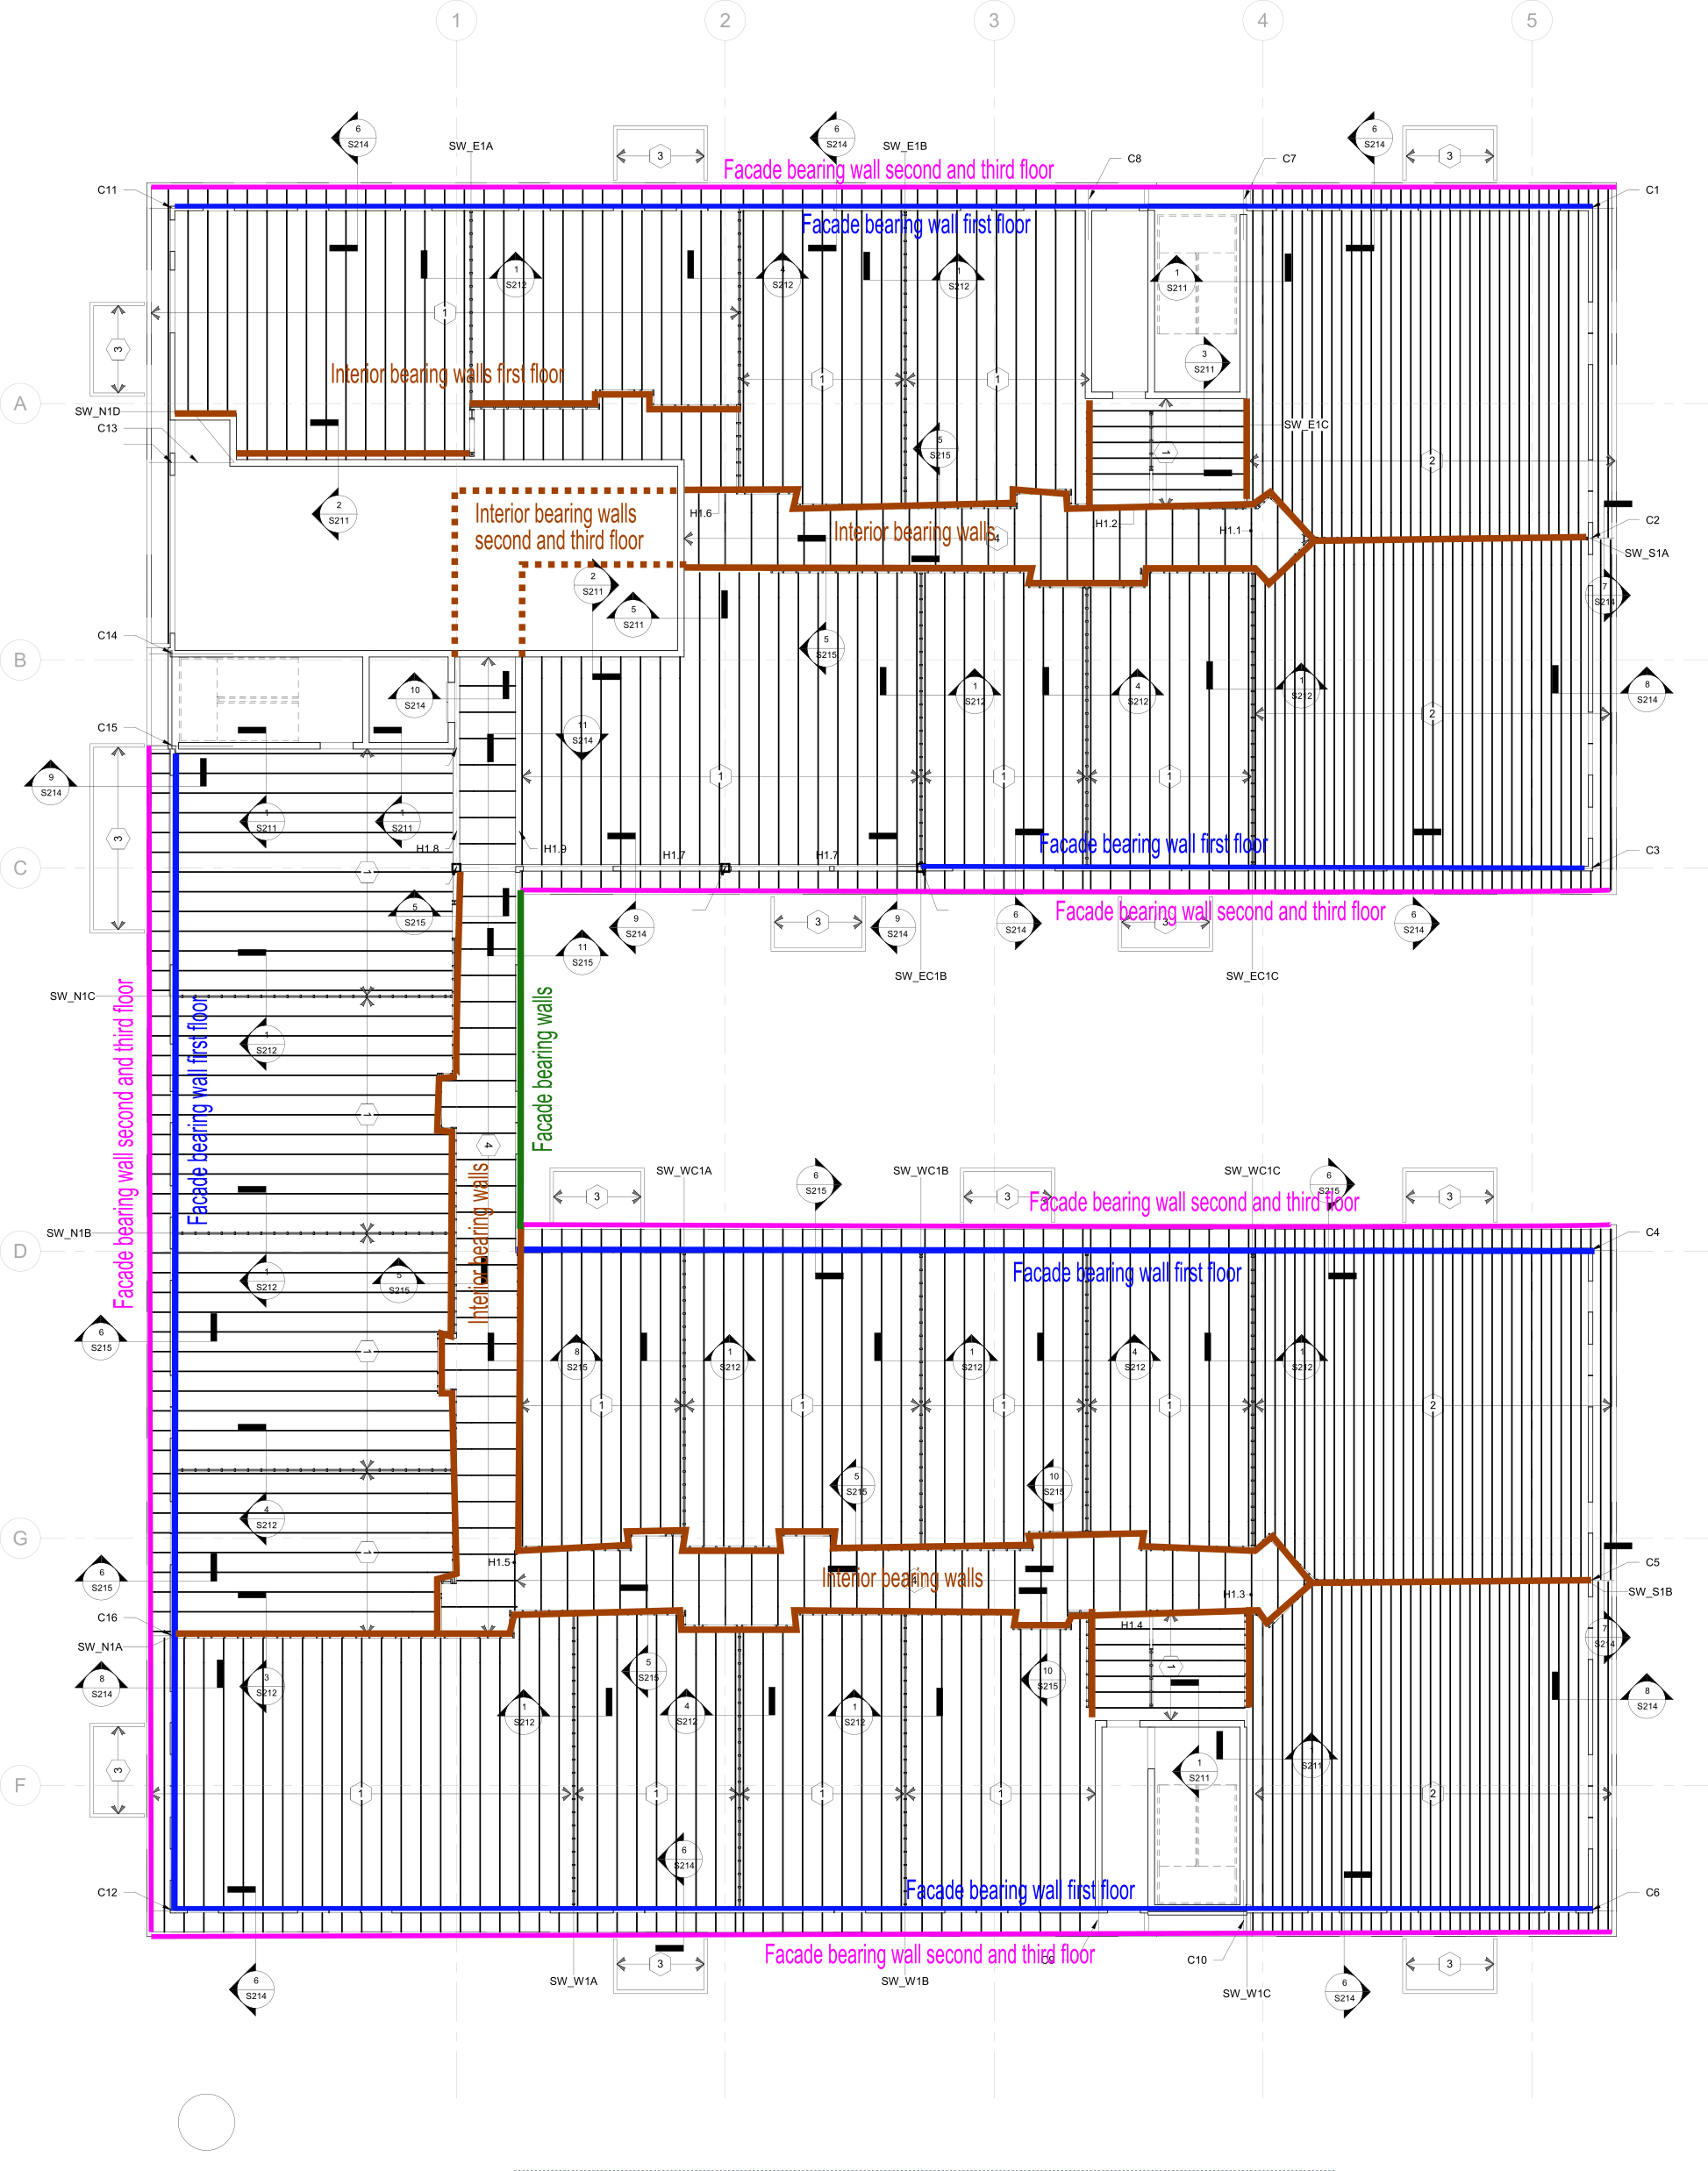
\includegraphics[width=120mm]{figures/bearing_walls_key_plan}
  \end{center}
  \caption{Bearing walls key plan. Roof}\label{fg_bearing_walls_key_plan}
\end{figure}

\subsubsection{Facade bearing walls at first floor}

\paragraph{Loads.}

\begin{itemize}
\item Vertical load from trusses: 43.34 kN/m
\item Vertical load on each stud: 10.57 kN
\item Wind load on stud height: 0.21 kN/m
\end{itemize}

\paragraph{Internal forces.}

\noindent Internal forces:

\begin{align}
  N_{max}&= 10.56\ kN \\
  M_{max}&= 0.18\ kN \cdot m
\end{align}

\paragraph{Bending and axial compression check.}

\subparagraph{Mechanical properties}

\begin{itemize}
\item Species: Hem-fir stud
\item Spacing: $0.24\ m$
\item Stud height: 2.64 m
\item Repetitive member factor: $C_r= 1.15$
\item Size factor: $C_F= 1.3$
\item $E_{min}= 3.03\ GPa$
\item $F'_c= 4.5\ MPa$.
\item $F'_b= 6.96\ MPa$.
\item Sections dimensions: (2x6''), effective (1.5x5.5'')= 38.1 x 139.7  mm.
\item Unbraced lenght x axis: 2.64 m
\item Unbraced lenght y axis: 0.3 m
\item Stud stability factor: $C_P= 0.68$
\end{itemize}

\begin{equation}
  N'_s= 23.94\ kN
\end{equation}

\noindent Capacity factor according to section 3.9.2 of NDS-2018 (equations 3.9.3 and 3.9.4):

\begin{equation}
  CF= 0.46 < 1 \implies OK
\end{equation}

\subsubsection{Facade bearing walls at second floor}

\paragraph{Loads.}

\begin{itemize}
\item Vertical load from trusses: 30.52 kN/m
\item Vertical load on each stud: 7.44 kN
\item Wind load on stud height: 0.21 kN/m
\end{itemize}

\paragraph{Internal forces.}

\noindent Internal forces:

\begin{align}
  N_{max}&= 7.44\ kN \\
  M_{max}&= 0.18\ kN \cdot m
\end{align}

\paragraph{Bending and axial compression check.}

\subparagraph{Mechanical properties}

\begin{itemize}
\item Species: Hem-fir stud
\item Spacing: $0.24\ m$
\item Stud height: 2.64 m
\item Repetitive member factor: $C_r= 1.15$
\item Size factor: $C_F= 1.3$
\item $E_{min}= 3.03\ GPa$
\item $F'_c= 4.5\ MPa$.
\item $F'_b= 6.96\ MPa$.
\item Sections dimensions: (2x6''), effective (1.5x5.5'')= 38.1 x 139.7  mm.
\item Unbraced lenght x axis: 2.64 m
\item Unbraced lenght y axis: 0.3 m
\item Stud stability factor: $C_P= 0.68$
\end{itemize}

\begin{equation}
  N'_s= 26.00\ kN
\end{equation}

\noindent Capacity factor according to section 3.9.2 of NDS-2018 (equations 3.9.3 and 3.9.4):

\begin{equation}
  CF= 0.34 < 1 \implies OK
\end{equation}

\subsubsection{Facade bearing walls at third floor}

\paragraph{Loads.}

\begin{itemize}
\item Vertical load from trusses: 16.01 kN/m
\item Vertical load on each stud: 7.81 kN
\item Wind load on stud height: 0.42 kN/m
\end{itemize}

\paragraph{Internal forces.}

\noindent Internal forces:

\begin{align}
  N_{max}&= 7.81\ kN \\
  M_{max}&= 0.36\ kN \cdot m
\end{align}

\paragraph{Bending and axial compression check.}

\subparagraph{Mechanical properties}

\begin{itemize}
\item Species: Hem-fir stud
\item Spacing: $0.49\ m$
\item Stud height: 2.64 m
\item Repetitive member factor: $C_r= 1.15$
\item Size factor: $C_F= 1.3$
\item $E_{min}= 3.03\ GPa$
\item $F'_c= 4.89\ MPa$.
\item $F'_b= 6.96\ MPa$.
\item Sections dimensions: (2x6''), effective (1.5x5.5'')= 38.1 x 139.7  mm.
\item Unbraced lenght x axis: 2.64 m
\item Unbraced lenght y axis: 0.3 m
\item Stud stability factor: $C_P= 0.68$
\end{itemize}

\begin{equation}
  N'_s= 26.00\ kN
\end{equation}

\noindent Capacity factor according to section 3.9.2 of NDS-2018 (equations 3.9.3 and 3.9.4):

\begin{equation}
  CF= 0.62 < 1 \implies OK
\end{equation}

\subsubsection{Interior bearing walls at first floor}

\paragraph{Loads.}

\begin{itemize}
\item Vertical load from trusses: 54.71 kN/m
\item Vertical load on each stud: 13.34 kN
\item Wind load on stud height: 0.0 kN/m
\end{itemize}

\paragraph{Internal forces.}

\noindent Internal forces:

\begin{align}
  N_{max}&= 13.34\ kN \\
  M_{max}&= 0.26\ kN \cdot m
\end{align}

\paragraph{Bending and axial compression check.}

\subparagraph{Mechanical properties}

\begin{itemize}
\item Species: Hem-fir stud
\item Spacing: $0.24\ m$
\item Stud height: 2.64 m
\item Repetitive member factor: $C_r= 1.15$
\item Size factor: $C_F= 1.3$
\item $E_{min}= 3.03\ GPa$
\item $F'_c= 4.89\ MPa$.
\item $F'_b= 6.96\ MPa$.
\item Sections dimensions: (2x6''), effective (1.5x5.5'')= 38.1 x 139.7  mm.
\item Unbraced lenght x axis: 2.64 m
\item Unbraced lenght y axis: 0.3 m
\item Stud stability factor: $C_P= 0.68$
\end{itemize}

\begin{equation}
  N'_s= 26.00\ kN
\end{equation}

\noindent Capacity factor according to section 3.9.2 of NDS-2018 (equations 3.9.3 and 3.9.4):

\begin{equation}
  CF= 0.74 < 1 \implies OK
\end{equation}

\subsubsection{Interior bearing walls at second floor}

\paragraph{Loads.}

\begin{itemize}
\item Vertical load from trusses: 36.3 kN/m
\item Vertical load on each stud: 17.70 kN
\item Wind load on stud height: 0.0 kN/m
\end{itemize}

\paragraph{Internal forces.}

\noindent Internal forces:

\begin{align}
  N_{max}&= 17.70\ kN \\
  M_{max}&= 0.35\ kN \cdot m
\end{align}

\paragraph{Bending and axial compression check.}

\subparagraph{Mechanical properties}

\begin{itemize}
\item Species: Hem-fir stud
\item Spacing: $0.24\ m$
\item Stud height: 2.64 m
\item Repetitive member factor: $C_r= 1.15$
\item Size factor: $C_F= 1.3$
\item $E_{min}= 3.03\ GPa$
\item $F'_c= 4.89\ MPa$.
\item $F'_b= 6.96\ MPa$.
\item Sections dimensions: (2x6''), effective (1.5x5.5'')= 38.1 x 139.7  mm.
\item Unbraced lenght x axis: 2.64 m
\item Unbraced lenght y axis: 0.3 m
\item Stud stability factor: $C_P= 0.68$
\end{itemize}

\begin{equation}
  N'_s= 26.00\ kN
\end{equation}

\noindent Capacity factor according to section 3.9.2 of NDS-2018 (equations 3.9.3 and 3.9.4):

\begin{equation}
  CF= 0.38 < 1 \implies OK
\end{equation}

\subsubsection{Interior bearing walls at third floor}

\paragraph{Loads.}

\begin{itemize}
\item Vertical load from trusses: 19.37 kN/m
\item Vertical load on each stud: 9.45 kN
\item Wind load on stud height: 0.0 kN/m
\end{itemize}

\paragraph{Internal forces.}

\noindent Internal forces:

\begin{align}
  N_{max}&= 19.37\ kN \\
  M_{max}&= 0.19\ kN \cdot m
\end{align}

\paragraph{Bending and axial compression check.}

\subparagraph{Mechanical properties}

\begin{itemize}
\item Species: Hem-fir stud
\item Spacing: $0.49\ m$
\item Stud height: 2.64 m
\item Repetitive member factor: $C_r= 1.15$
\item Size factor: $C_F= 1.3$
\item $E_{min}= 3.03\ GPa$
\item $F'_c= 4.89\ MPa$.
\item $F'_b= 6.96\ MPa$.
\item Sections dimensions: (2x6''), effective (1.5x5.5'')= 38.1 x 139.7  mm.
\item Unbraced lenght x axis: 2.64 m
\item Unbraced lenght y axis: 0.3 m
\item Stud stability factor: $C_P= 0.68$
\end{itemize}

\begin{equation}
  N'_s= 26.00\ kN
\end{equation}

\noindent Capacity factor according to section 3.9.2 of NDS-2018 (equations 3.9.3 and 3.9.4):

\begin{equation}
  CF= 0.43 < 1 \implies OK
\end{equation}
